% \begin{itemize}
%     \item \textbf{Question:}
%     \item \textbf{Answer:}
% \end{itemize}
\section{Lecture Notes Section 8.1}\label{sec:model_explanation}
\subsection{8.1.2 Conditional probability}
Suppose you have a space, called bAgOfFriEs, the space represents a bag of fries. Barry added ketchup(A) and mayonaise(B). Now Sjonnie, is eating the first fry. Now Ingrid wants to know whether the occurence of ketchup(A) and mayonaise(B) are independent or not. To determine whether Ketchup(A) depends on mayonaise(B), she must calculate, the probability of first picking a frie with ketchup(A) and mayonaise(B) and then determining how large that probability is as a fraction of picking any frie that has some mayonaise(B) on it (regardles of whether it has ketchup(A) or not).
\begin{enumerate}
    \item p(A|B)=P(AB)/P(B)=A depends on B = the probability that Ketchup(B) depends on mayonaise(B).
    \item p(B|A)=P(AB)/P(A)=B depends on A = the probability that mayonaise(B) depends on ketchup(A).
\end{enumerate}
So looking at Venn diagram, conditional probability of an option is a fraction, and hence probability that looks at: how big is the overlap of the 2 options divided by the total probability of one single option. That is why conditional probability of 2 events can be expressed for two scenarios, (A depends on B, or vice versa).


If A and B completely overlap, the conditional probability = 1. That means they are INDEPENDENT. 
\subsection{question}
The independence is a bit weird because if p(AB)=0.98 and P(B)=0.99 {P(A)=0.99)} then there is a $\frac{0.98}{0.99}=0.989$ probability that A depends on B, but if it shifts over even more, to a higher probability of A depending on B, eventually, suddenly they are independent.

\subsection{8.1.3 Bayes Theorem}
Nothing offensive, "Bobby's Bits" or something, has 3 production machines,1,2 and 3. 
\begin{enumerate}
    \item machine builds 20\%:$p(A_1)=0.2$, fails 5\% of its products $p(B|A_1)=0.05$ 
    \item machine builds 30\%$p(A_2)=0.3$, fails 3\% of its products$p(B|A_2)=0.03$
    \item machine builds 50\%$p(A_3)=0.5$, fails 1\% of its products$p(B|A_3)=0.01$
\end{enumerate}
Now given one product failed, what are the odds \st{you send back the cheque for 25 pound from the other company name - saying "We're sorry," we couldn't get the supplies from America because they ran out of sock.} that the failed product came out of machine "i"?

\subsubsection{Attempt solution using bayes formula} 
\begin{equation}
    P(A|B)=\frac{p(A)p(B|A)}{P(B)}
\end{equation}
The question asks: given P(B), what is the probability that it was machine i. That comes down to: 
\begin{figure}
    \centering
    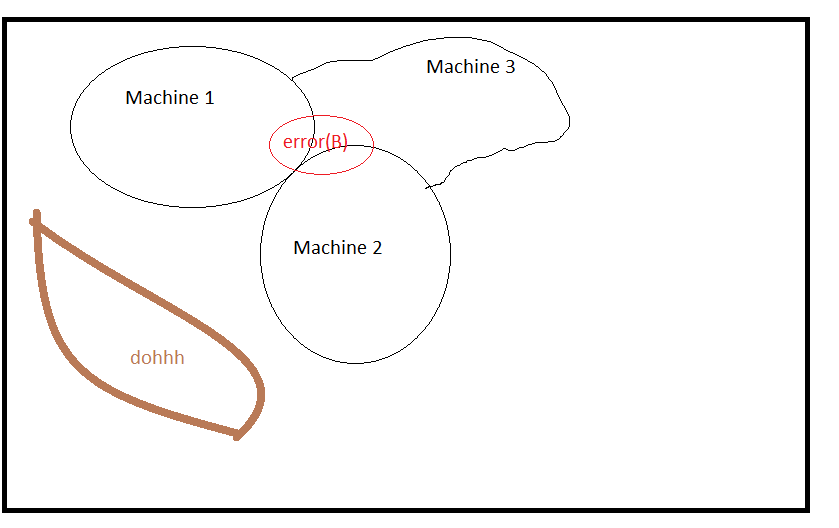
\includegraphics{images/lectureNotes8_1_3_Bayes.png}
    \caption{Visualisation machines as homer}
    \label{fig:my_label}
\end{figure}
Now the probability that an error occurs is: 
\begin{equation}
    \sum_{i=1}^2 p(A_i)\cdot p(B_i)=0.2\cdot 0.05+0.3\cdot 0.03+0.5\cdot0.01=0.024
    \label{eq:prob_error}
\end{equation}
and the probability that "that"=already known, error is from machine 1, is:
\begin{equation}
    \frac{\text{probability of error of machine i}}{\text{total probability of error}}
    \label{eq:human_prob_error_of_machine}
\end{equation}
or expressed as formula:
\begin{equation}
    \frac{p(A_1)p(B_1)}{\sum_{i=1}^2 p(A_i)\cdot p(B_i)}=\frac{0.2*0.05}{0.024}=0.41666
    \label{eq:prob_error_of_machine}
\end{equation}
Now the formal notation of \cref{eq:prob_error} is:
\begin{equation}
    p(B):=sum_i^3 p(B|A_i)\cdot p(A_i)
\end{equation}
And the notation of: given event B, the probability that it is A, as computed in \cref{eq:human_prob_error_of_machine} and \cref{eq:human_prob_error_of_machine}, is:
\begin{equation}
    p(A_1|B)=\frac{p(B|A1)\cdot p(A_1)}{p(B)}=\frac{0.05\cdot 0.2}{0.024}=0.4166
\end{equation}
As you can see the formal notation is the same as the intuitive computation. You can also put this in matlab


\newpage
\section{Bonus:Section 8.4 Covariance Analysis}


\begin{itemize}
    \item \textbf{Question:} Is the expected value of a matrix (always) a matrix (in equation 8.27)?
    \item \textbf{Answer:}
\end{itemize}

\begin{itemize}
    \item \textbf{Question:} How do you actually compute the expected value of a matrix (in equation 8.27)?
    \item \textbf{Answer:}
\end{itemize}

\subsection{Variance of a vector $x$ with $n$ dimensions}
Suppose the following vector $x=$ with $n$ dimensions:
\begin{equation}
x=
    \begin{bmatrix}
    6\\
    5\\
    4\\
    \end{bmatrix}
\end{equation}
\subsubsection{Mean $\mu$}
Then the mean of that vector:
\begin{equation}
    \mu_x =\frac{\sum_{i=1}^{i=n}{x_i}}{n}= \frac{\sum_{i=0}^{i=n-1}{x_i}}{n}=
\end{equation}
\begin{equation}
    \mu_x=\frac{6+5+4}{3}=\frac{15}{3}=5
\end{equation}
\subsubsection{Variance}
The variance is the average squared distance from the mean.
\begin{equation}
    \sigma_x=\frac{1}{n}\sum_{i=1}^{i=n}{({x_i}-\mu_x)}^2=
\end{equation}
\begin{equation}
    \sigma_x=\frac{1}{3}({(6-5)}^2+{(5-5)}^2+{(4-5)}^2)=
\end{equation}
\begin{equation}
    \sigma_x=\frac{1}{3}({(1)}^2+{(0)}^2+{(-1)}^2)=
\end{equation}
\begin{equation}
    \sigma_x=\frac{1}{3}(2)=\frac{2}{3}
\end{equation}
\subsubsection{Standard deviation $\sigma$}
And the standard deviation is (the root of the variance):
\begin{equation}
    \sigma_x=\sqrt{\frac{1}{n}\sum_{i=1}^{i=n}{({x_i}-\mu_x)}^2}=
\end{equation}
\begin{equation}
    \sigma_x=\sqrt{\frac{1}{3}({(6-5)}^2+{(5-5)}^2+{(4-5)}^2)}=
\end{equation}
\begin{equation}
    \sigma_x=\sqrt{\frac{1}{3}({(1)}^2+{(0)}^2+{(-1)}^2)}=
\end{equation}
\begin{equation}
    \sigma_x=\sqrt{\frac{1}{3}(2)}=\sqrt{\frac{2}{3}}
\end{equation}
\subsubsection{correlation $\rho_{xy}$}
The correlation is computed between two datasets$/$vectors. Now computing the correlation between $\bar{x}$ and $\bar{x}$ should return one, it's a good exercise but at the same time a bit like:
\begin{figure}
    \centering
    
\includegraphics{images/lion.jpg}
    \caption{Computing the correlation of of a single vector with itself.}
    \label{fig:my_label}
\end{figure}
So lets imagine another vector $\bar{y}$:
\begin{enumerate}
    \item Vector $\bar{y}$
        \begin{equation}
            \bar{y}=
            \begin{bmatrix}
            6\\
            1\\
            2\\
            \end{bmatrix}
        \end{equation}
    \item \textbf{Mean $\mu_y$}
        Then the mean of that vector:
        \begin{equation}
            \mu_y =\frac{\sum_{i=1}^{i=n}{x_i}}{n}= \frac{\sum_{i=0}^{i=n-1}{x_i}}{n}=
        \end{equation}
        \begin{equation}
            \mu_y=\frac{6+1+2}{3}=\frac{9}{3}=3
        \end{equation}
    \item \textbf{Variance}
        The variance is the average squared distance from the mean.
        \begin{equation}
            \sigma_y=\frac{1}{n}\sum_{i=1}^{i=n}{({x_i}-\mu_x)}^2=
        \end{equation}
        \begin{equation}
            \sigma_y=\frac{1}{3}({(6-3)}^2+{(1-3)}^2+{(2-3)}^2)=
        \end{equation}
        \begin{equation}
            \sigma_y=\frac{1}{3}({(3)}^2+{(-2)}^2+{(-1)}^2)=
        \end{equation}
        \begin{equation}
            \sigma_y=\frac{1}{3}(14)=\frac{14}{3}
        \end{equation}
    \item \textbf{Standard deviation $\sigma$}
        And the standard deviation is (the root of the variance):
        \begin{equation}
            \sigma_y=\sqrt{\frac{1}{3}(14)}=\sqrt{\frac{14}{3}}
        \end{equation}
\end{enumerate}
Now the correlation between $\bar{x}$ and $\bar{y}$ can be computed with:
\begin{equation}
    \rho_{xy}=\frac{E[(X-E(Y))(Y-E(Y))]}{\sqrt{E{[{(X-E(Y))}^2E[{(Y-E(Y))}^2]}}}=\frac{\sigma_{xy}}{\sigma_x\sigma_y}=
\end{equation}
Where $\sigma_{xy}=covariance(\bar{x},\bar{y})$  So:
\begin{equation}
    \rho_{xy}=\frac{E[(X-E(Y))(Y-E(Y))]}{\sqrt{E{[{(X-E(Y))}^2E[{(Y-E(Y))}^2]}}}=\frac{\sigma_{xy}}{\sigma_x\sigma_y}=\frac{\mu_{xy}}{\sigma_x\sigma_y}=\frac{covariance(\bar{x},\bar{y})}{\sigma_x\sigma_y}
\end{equation}
From this equation you can derive that the correlation should always be $-1\leq \rho_{xy} \leq 1$

Filling in the numbers yields:
\begin{equation}
    \rho_{xy}=\frac{\frac{5+3}{2}}{\sqrt{\frac{2}{3}}\frac{14}{3}}=\frac{56\sqrt{6}}{9}=15.2413
\end{equation}

\subsubsection{covariance $P_{x}$}
You can compute the covariance of a single vector $\bar{x}$ with $n=3$ dimensions as:
\begin{equation}
    P_x=
    \begin{bmatrix}
            \sigma_{1,1} & \rho_{2,1}\sigma_{2}\sigma_{1} &\rho_{n,1}\sigma_{n}\sigma_{1}\\
            \rho_{1,2}\sigma_{1}\sigma_{2} & \rho_{2,2}\sigma_{2}\sigma_{2} &\rho_{n,2}\sigma_{n}\sigma_{2}\\
            \rho_{1,n}\sigma_{1}\sigma_{n} & \rho_{2,n}\sigma_{2}\sigma_{n} &\rho_{n,n}\sigma_{n}\sigma_{n}\\
    \end{bmatrix}
\end{equation}
Where
\begin{enumerate}
    \item $\sigma_{1,1}$= $E[(X_1)-E[X_1])(X_1)-E[X_1])]$ \cite{covariance_matrix}
\end{enumerate}
\textbf{    \begin{itemize}
        \item \textbf{Question:} How do you fill that in for a single vector? What is $\sigma_11$?
        \item \textbf{Answer:}
    \end{itemize}}
According to \cite{covariance_stack} the covariance of a single vector can also be computed with:
\begin{equation}
	cov(\bar{x},\bar{y})=\frac{1}{n-1}\sum_{i=1}^{i=n}(x_i-\mu_x)(y_i-\mu_y)
\end{equation}

\subsubsection{covariance $P_{xy}$}
According to \cite{covariance_stack} To compute the covariance-variance matrix, of a vector $X$ with $n$ entries you use the covariance of the vectors (a scalar) in the following equation:
\begin{equation}
	\begin{bmatrix}
		{\sigma_x}^2 & cov(x,y)\\
		cov(x,y) & {\sigma_y}^2\\
	\end{bmatrix}
\end{equation}


\newpage
\section{Bonus:Section 8.5 Least squares method}
Suppose you want to estimate the amount of socks going to the parallel universe in the washing machine; $\Bar{y}$ based on the number of handstands people do per week $\Bar{x}$. 
\begin{enumerate}
    \item The observation comes from the parallel universe denoted with $\mathbb{V}$. This parallel universe $\mathbb{V}$ is only connected to dishwashers of a certain brand and type, so that the people using those washing machines are less likely to find other people with the same problem and will doubt themselves. In total, 93.034 washing machines were made of this brand and type, of which $m=42$ are connected to the parallel universe. One can say, the parallel universe $\mathbb{V}$ has $m$ dimensions/stations where they count how many socks came in. In other words $y \in \mathbb{V}^m$.
    \item Now, the sock brokers of the parallel dimension always try to predict how many socks will be coming in, they indicate their belief in the amount of incoming socks with a few numbers. To be exact they predict it with $n$ numbers  in vector $\Bar{x}$. In other words, $x \in \mathbb{V}^n$.
    \item But then there's the SEC that checks the behaviour of the sock brokers, if their predictions are too far off, the negatively influence the sockonomy. The SEC publishes their numbers on how well the sock brokers predict the nr of counted socks that come into the parallel dimension, ACCORDING TO THE COUNTERS, in the residuals vector $\epsilon$, sometimes misleadingly called error. But they just sit right next to the incoming sock counting stations an report per station what the difference between the counted incoming amount of socks, and some report of the sock brokers is. So they produce as much numbers as stations = $m$. In other words $\Bar{\epsilon}\in\mathbb{V}^m$. 
    \item As you might have noticed, there's a difference between the belief in the number of numbers that the sock brokers shout, and the nr of actual incoming-sock-counting-stations. Therefore, there's a large IT firm that conveniently converts the belief of the sock brokers, into a number of expected socks incoming. Their work is a set of numbers, called matrix A. Their work takes in $n$ numbers, and outputs $m$ numbers, therefore, $A$ is an $n\cdot m$ matrix. This matrix is accordingly called: \textit{design-matrix} or \textit{information-matrix}.
    \item Now assume a linear relation between the the incoming socks and the belief of in the nr of incoming socks is linear.
    \item Now the workers at the counting stations are being strictly monitored, whether they do not steal any socks, and whether they don't accidentally make counting mistakes (count a sock extra). However, sometimes they do make "mistakes", these mistakes are monitored by the galactic- overlords and overladies in matrix $P_{yy}$. I don't know how many numbers it has. Additionally this is most likely a candidate for the TRUE ERROR.
    \begin{itemize}
        \item \textbf{Question:} What are the dimensions of matrix $P_{yy}$?
        \item \textbf{Answer:}
    \end{itemize}
\end{enumerate}
\subsection{Finding a solution to the Least Squared Problem}
A solution in this context, is optimal performance of the sock brokers $\Bar{x}$ with a prediction, that, after processing of their belief/prediction by the IT company $\Bar{A}$ corresponds as close as possible to actual incoming nr of socks counted at each individual counting station $\Bar{y}$. This situation means the square of the residual $\epsilon$ is minimised
\begin{enumerate}
    \item (It's square, cause if $\epsilon$ should be as low as possible you could just do -100000, but then you'll grossly underestimate the actual nr of socks. It shouldn't be too far below nor to far over.)
    \item Furthermore, it's not good enough to just get the nr. of summed socks of all counting stations predicted correcty, you can say everything comes in at station 1, but then you'll (unless they actually do) have 42 wrong predictions. So really the brokers have to predict, through the IT company, the exact nr of incoming socks counted at each individual counting station.
\end{enumerate}
So to do this the governing body of the parallel universe tries to find a solution where:
\newline
\text{the nr of counted socks per counting station n}\newline
= \newline
\text{The belief in the nr of socks by the sock brokers}\newline 
$\cdot$
\newline 
\text{converted to a prediction of nr of socks per counting station by the IT company}
\newline
+
\newline
\text{the mistakes and thefts of the counters}
\newline
\newline
Or in mathematical terms:
\begin{equation}
\Bar{y}=A\Bar{x}+\epsilon
\label{eq:observations_vs_parameter}
\end{equation}
Since, the governing body wants to minimise the square of the residuals $\epsilon$, they minimize the cross product of the transpose $\epsilon^t$ times $\epsilon$:
\begin{equation}
    J=\epsilon^t\epsilon
    \label{eq:squared_error}
\end{equation}  
\begin{itemize}
    \item \textbf{Question:} is the multiplication of the residual a cross product or dotproduct multiplication?
    \item \textbf{Answer:}
\end{itemize}

\noindent Now you can rewrite \cref{eq:observations_vs_parameter} to:
\begin{equation}
    \Bar{\epsilon}=\Bar{y}-A\cdot\Bar{x}
    \label{eq:epsilon_rewritten}
\end{equation}
\begin{itemize}
    \item \textbf{Question:}is it indeed a dot product between $A$ and $\Bar{x}$
    \item \textbf{Answer:}
\end{itemize}
and substitute \cref{eq:epsilon_rewritten} into \cref{eq:squared_error}. Yielding:
\begin{equation}
    J={(\Bar{y}-A\cdot\Bar{x})}^t\cdot(\Bar{y}-A\cdot\Bar{x}) =
\end{equation}

\begin{equation}
    J={(\Bar{y}^t-A^t\cdot\Bar{x}^t)}\cdot(\Bar{y}-A\cdot\Bar{x}) =
\end{equation}

\begin{equation}
    J=\Bar{y}^t(\Bar{y}-A\Bar{x})-A^t\Bar{x}^t(\Bar{y}-A\cdot\Bar{x}) =
    \label{eq:cost_function}
\end{equation}

Now for a reason currently unknown, the sock brokers can't minimise the LHS term, so must optimise the RHS term. They also can't just set their belief $\Bar{x}$ to 0.
\begin{itemize}
    \item \textbf{Question:}Why can't the first term be minimised when $A\hat{x}$ approximates $\Bar{y}$ in eq 8.39? That appears to be a minimisation of the LHS term.
    \item \textbf{Answer:}
\end{itemize}
So the sock brokers try to minimize $J$ by minimizing the RHS term without setting $\Bar{x}$ to 0. The optimal solution is denoted with $\hat{x}$. That leads to:
\begin{equation}
    \hat{x}^tA^t(\Bar{y}-A\hat{x})=0
\end{equation}
Dividing both sides by $\hat{x}$:
\begin{equation}
    A^t(\Bar{y}-A\hat{x})=0
\end{equation}
Which can be written to the so-called normal equations:
\begin{equation}
    A^t\Bar{y}=AA^t\hat{x}
\end{equation}
\begin{equation}
    \hat{x}=\frac{A^t\Bar{y}}{=AA^t}
    \label{eq:broker_solution}
\end{equation}
\begin{itemize}
    \item 
    Since the sock brokers did not get any information on the actual mistakes of the counting stations from the galactic- overladies and overlords, they did not give any more importance to specific numbers in their belief vector $\bar{x}$ to compensate those mistakes that would be listed in $P_{yy}$. So the prediction/solution of the sock brokers is unweighted.
    \item $A^tA$ is called the normal matrix 
    \item $\Bar{x}$ is called the unweighted solution because no info of $P_{yy}$ is used,($P_{yy}$ is the identity matrix in that/this case).
\end{itemize}
\subsection{Using the galactic- overladies' and overlords' counter mistake data $P_{yy}$}
If you get that insider information of the galactic- overladies and overlords, the sock brokers can optimize their solution/estimate on the number of socks that will be counted by incorporating that insider information $P_{yy}$ in their cost function. They minimize (Please note the inverse of $P_{yy}$ instead of the transpose!):

\begin{equation}
    J_{inside information}=\bar{\epsilon}^tP_{yy}^-1\bar{\epsilon}
\end{equation}

\begin{itemize}
    \item \textbf{Question:} is ${P_{yy}}^{-1}$ the same as the inverse of $P_{yy}$?
    \item \textbf{Answer:}
\end{itemize}

\begin{itemize}
    \item \textbf{Question:} Why do they multiply with the inverse** of $P_{yy}$ instead of $P_{yy}$?
    ** see question above
    \item \textbf{Answer:}
\end{itemize}

They repeat their computations as listed in \cref{eq:epsilon_rewritten} to \cref{eq:broker_solution} and find the weight solution/estimate of the least squares problem:
\begin{equation}
    \hat{x}={(A{P_{yy}}^{-1}A^t)}^{-1}{A^t{P_{yy}}^{-1}\Bar{y}}
    \label{eq:insider_broker_solution}
\end{equation}

\subsection{Reduction dataset of the nr of counted socks}
A special dataset of the number of counted socks at the counting stations can be directly computed at the grace of the galactic- overlords and ladies. This list of number of socks is not called $\bar{y}$ but $\bar{y}^*$. Where $\bar{y}^*={P_{yy}}^{-\frac{1}{2}}$

\begin{itemize}
    \item \textbf{Question:}The text says: "If your pc can't compute a covariance matrix of the observations. What is the covariance matrix in this whole ordeal? $P_{yy}$?
    \item \textbf{Answer:}Almost. $P_{xx}$ is the covariance matrix of $\bar{x}$ and $P_{yy}$ is the covariance matrix of $\bar{y}$. Source: section 8.4.3
\end{itemize}

\newpage
\section{8.7 Properties of the least squares algorithm}
\begin{enumerate}
    \item The inverse of the normal matrix becomes the covariance matrix of the estimated parameters. Written in formulas:
    \begin{itemize}
        \item the inverse of the normal matrix = ${(AA^t)}^{-1}$
        \item the estimated parameters $\bar{x}$
        \item the covariance matrix of the estimated parameters = $P_{xx}$. Source: given in as definition of section 8.4.3
        \item hence: ${(AA^t)}^{-1}=P_{xx}$
    \end{itemize}
\end{enumerate}

\subsection{8.5.1 Parameter Covariance matrix}
So the Galactic- overladies and overlords get that inside information on the mistakes that are being made in each of the sock counting stations, this information is presented as the covariance matrix $P_{yy}$ of the actual number of counted incoming socks $\bar{y}$.Now there also exists a covariance matrix for the belief $\bar{x}$ in the nr of counted incoming stocks of the sock brokers. This covariance matrix is named: $P_{xx}$. It just so happends that this covariance matrix can be computed using the conversion matrix of the IT company. First take the unweighted estimate of the stock brokers.

\begin{equation}
    \hat{x}   = {(A^tA)}^{-1}A^t\bar{y}=B\bar{y}
\end{equation}
Then: 
\begin{equation}
    P_{xx}=BB^t
\end{equation}
Or
\begin{equation}
    P_{xx}={(A^tA)}^{-1}A^tA{(A^tA)}^{-1}
\end{equation}
Something to the power of $-1$ times something = 1 hence:
\begin{equation}
    P_{xx}={(A^tA)}^{-1}
\end{equation}

\begin{itemize}
    \item \textbf{Question:} given \cref{fig:covariance}, is the covariance of $\bar{x}$, if it has 3 numbers in it, a 2d picture, with on the x axis vector element 0,1 and 2 and on the y-axis the (absolute) magnitude of these vector elements? E.g. $\bar{x}=[4.5,20,83.5]$ (with large positive covariance).
    \item \textbf{Answer:}
\end{itemize}
\begin{figure}
    \centering
    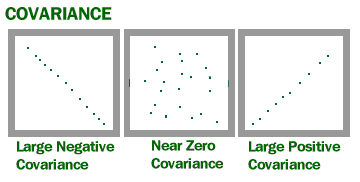
\includegraphics{images/covariance.png}
    \caption{Visualisation of covariance}
    \label{fig:covariance}
\end{figure}


\subsection{8.7.1 Effects of scaling}
The information on the amount of mistakes at each individual counting station, as provided by the galactic- overlords and overladies, $P_{yy}$ was a matrix. When it is mid-summer, counters have a vitamin D shortage since their sun, Becelproactief, is covered by a gas cloud that reduces the amount of incoming light. This vitamin deficiency causes an increased mistake rate of the counters. This increased rate of error can be called scaling, and is indicated with the number $\lambda$. 

Now a peculiar thing happens, the sock brokers are not able to use this scaling, as everytime they try to enter it in their broker solution/estimate of the number of socks, with the galactic- overlords' and ladies' error information with included scaling: $P_{yy}=\lambda I$ , it drops out. Watch:


\begin{itemize}
    \item \textbf{Question:} is $\lambda$ a vector or a scalar?
    \item \textbf{Answer:}
\end{itemize}

\begin{equation}
    \hat{x}={(A{P_{yy}}^{-1}A^t)}^{-1}{A^t{P_{yy}}^{-1}\Bar{y}}
    \label{eq:insider_broker_solution}
\end{equation}

\begin{equation}
    \hat{x}={(A{(\lambda I)}^{-1}A^t)}^{-1}{A^t{(\lambda I)}^{-1}\Bar{y}}
    \label{eq:insider_broker_solution}
\end{equation}
*The inverse of the inverse of $(\lambda I)$ multiplied with the inverse of $(\lambda I)$ = 1, hence:
\begin{equation}
    \hat{x}={(AA^t)}^{-1}{A^t\Bar{y}}
    \label{eq:insider_broker_solution}
\end{equation}

\begin{itemize}
    \item \textbf{Question:} What is the difference between the inverse of a matrix and 1 divided by a matrix?
    \item \textbf{Answer:}
\end{itemize}
 So to conclude, the scaling does not affect the sock brokers prediction.
\subsubsection{Scaling on the sock brokers covariance matrix}
Do you remember the covariance matrix of the sock brokers belief $\hat{x}$ in the nr of counted incoming stocks $\bar{y}$? Well, neither do I but that covariance matrix is influenced by the scaling:
\begin{equation}
    P_{xx}=\lambda{(A^tA)}^{-1}
\end{equation}
That means if there is scaling, the covariance of $\bar{x}$ is affected. This somehow is a problem, so there are techniques that calibrate the variance, which are referenced in source[30].

\begin{itemize}
    \item \textbf{Question:} Why does one want a covariance matrix of $\bar{x}$ that is independent of scaling effects? What is it used for?
    \item \textbf{Answer:}
\end{itemize}


\begin{itemize}
    \item \textbf{Question:} Why does the variance of $\bar{x}$ need to be calibrated??
    \item \textbf{Answer:}
\end{itemize}

\subsection{8.72 Penrose-More pseudo inverse, sounds gnarly}
Sir Roger Penrose is a famous Mathematician, known for his highly controversial book, Shadows of the Mind, and nowadays focuses on testable hypothesis that are frowned upon by the scientific community in the Penrose institute. Apparently the boffin also did something for the Least squares solution strategies.

Remember how the sock brokers expressed their belief in the nr of incoming socks per station with a vector $\bar{x}$ containing $m$ numbers (hence of dimension $m$)? But how there were actually $n$ counting stations, and how the IT company had to translate that discrepancy? Well, the IT company has 3 strategies:
\begin{enumerate}
    \item $\hat{x}={(A^tA)}^{-1}A^t\bar{y}=K\bar{y} \  \forall \ m>n$
    \item $\hat{x}={A}^{-1}\bar{y} \  \forall \ m=n$
    \item $\hat{x}=A^t{(AA^t)}^{-1}\bar{y} \  \forall \ m<n$
\end{enumerate}
\begin{itemize}
    \item \textbf{Question:}Why is the middel/2nd solution considered trivial?
    \item \textbf{Answer:}
\end{itemize}

\begin{itemize}
    \item \textbf{Question:}In Eq 8.58 why is $AK-I=0$?
    \item \textbf{Answer:}
\end{itemize}

Now this K is called the Kalman gain matrix, or K, or called pseudo-inverse of $A$, or Penrose-Moore pseudoinverse of $A$, which in literature is also written as $A^+$.
However, you don't have to worry about the dimensions $m$ and $n$ because Matlab automatically selects whichever of the 2 solution strategies if $m\neq n$ is appropriate when doing an LS problem.
\begin{itemize}
    \item \textbf{Question:} What does it mean Matlab automatically selects the ?
    \item \textbf{Answer:}
\end{itemize}



